\documentclass{iopconfser}
\usepackage{float}
\usepackage{graphicx}
\usepackage{subcaption}
\usepackage[automake]{glossaries-extra}
\usepackage{ragged2e}
\usepackage[export]{adjustbox}
\usepackage{mathtools}
\usepackage{setspace}
\usepackage{dirtytalk}

\onehalfspacing
% \makeglossaries

\setabbreviationstyle[acronym]{long-postshort-user}
\glssetcategoryattribute{acronym}{nohyperfirst}{true}
\setabbreviationstyle{short-nolong}
\makeglossaries

% --------------------
% ---- Glossaries ----
% --------------------
\newglossaryentry{asyncio}{name=Asyncio, description={A Python library for asynchronous code.}}
\newglossaryentry{stim}{name=STIM300, description={A MEMS-based \gls{imu}}}
\newglossaryentry{f9p}{name=F9P, description={A Global Navigation Satellite System (GNSS) receiver manufactured by u-blox.}}

% --------------------
% ----- Acronyms -----
% --------------------
\newacronym{asv}{ASV}{Autonomous Surface Vehicle}
\newacronym{dolp}{DoLP}{Degree of Linear Polarization}
\newacronym{aolp}{AoLP}{Angle of Linear Polarization}
\newacronym{sitaw}{SITAW}{Situational Awareness}
\newacronym{poe}{PoE}{Power over Ethernet}
\newacronym{pps}{PPS}{Pulse Per Second}
\newacronym{cpfa}{CPFA}{Color-Polarization Filter Array}
\newacronym{utc}{UTC}{Coordinated Universal Time}
\newacronym{imu}{IMU}{Inertial Measurement Unit}
\newacronym{tov}{TOV}{Time of Validity}
\newacronym{tm2}{TM2}{Time mark data}
\newacronym{gnss}{GNSS}{Global Navigation Satellite System}
\newacronym{ptp}{PTP}{Precision Time Protocol}

% \glsaddall
% \makenoidxglossaries

% \glsunset{cpu}
\glsunset{gnss}
\glsunset{imu}
\glsunset{tm2}
\glsunset{utc}

% --------------------
% ----- Shortcuts ----
% --------------------


\addbibresource{mylib.bib}


\begin{document}
\title{CASPAR: A CUDA Accelerator for Symbolic Programming with Adaptive Reordering}
\author{Emil Martens}

Mores law dead
Tradeoff between performance and complexity
Parallel computing and new algorithms
Symbolic computing offer new approach to computing.
One area is nonlinear optimization

\section{Introduction}

With Moore's law coming to an end, the industry has shifted its focus from increasing the clock speed of processors to increasing the number of cores.
GPUs are a prime example of this, with the number of cores increasing exponentially over the last decade.
New programming paradigms have emerged to take advantage of this, such as CUDA and OpenCL.
These paradigms allow for the programmer to write code that can be executed in parallel on the GPU, but it adds a layer of complexity to the programming process.
Application specific libraries have been developed to solve common problems, such as CuBlas for linear algebra, and higher order frameworks have been developed to abstract the complexity of GPU programming, such as PyTorch for machine learning.


\section{Background}

\subsection{Nonlinear Optimization}
Talk about the BAL papers.
\gls{pcgnr}



\subsection{Lie Algebra}
Talk about micro lie theory and symforce.

\subsection{GPU Computing}
Fast but dumb.
\section{Symbolic Computing}
\subsection{Limitations of Existing}
\gls{symengine} and \gls{sympy} are great for mathematics but not for generating high performance code.

\subsubsection{Multiple Outputs}
Vector instructions.
SinCos.

\subsubsection{Context Awareness}
a/x -> a/x,   a/x, b/x -> r = 1/x, a*r, b*r

\subsection{Hardware Oriented Code Generation}
Use available acceleratost, e.g. norm functions.


\subsection{Adaptive Reordering}
Each thread on the GPU has a finite set of 32-bit registers available.
If a kernel need more registers than whats available, local memory is used.
Ther is called register spilling an has a negative on performance, as local memory is as slow as global memory.
To minimize the amount of register spilling we want to find an optimal expression ordering.
This problem is called the bandwidth minimization problem and is NP-hard.
\begin{figure}[H]
    \centering
    \begin{tabular}[b]{ccc}

        \subcaptionbox{Array of scalars}{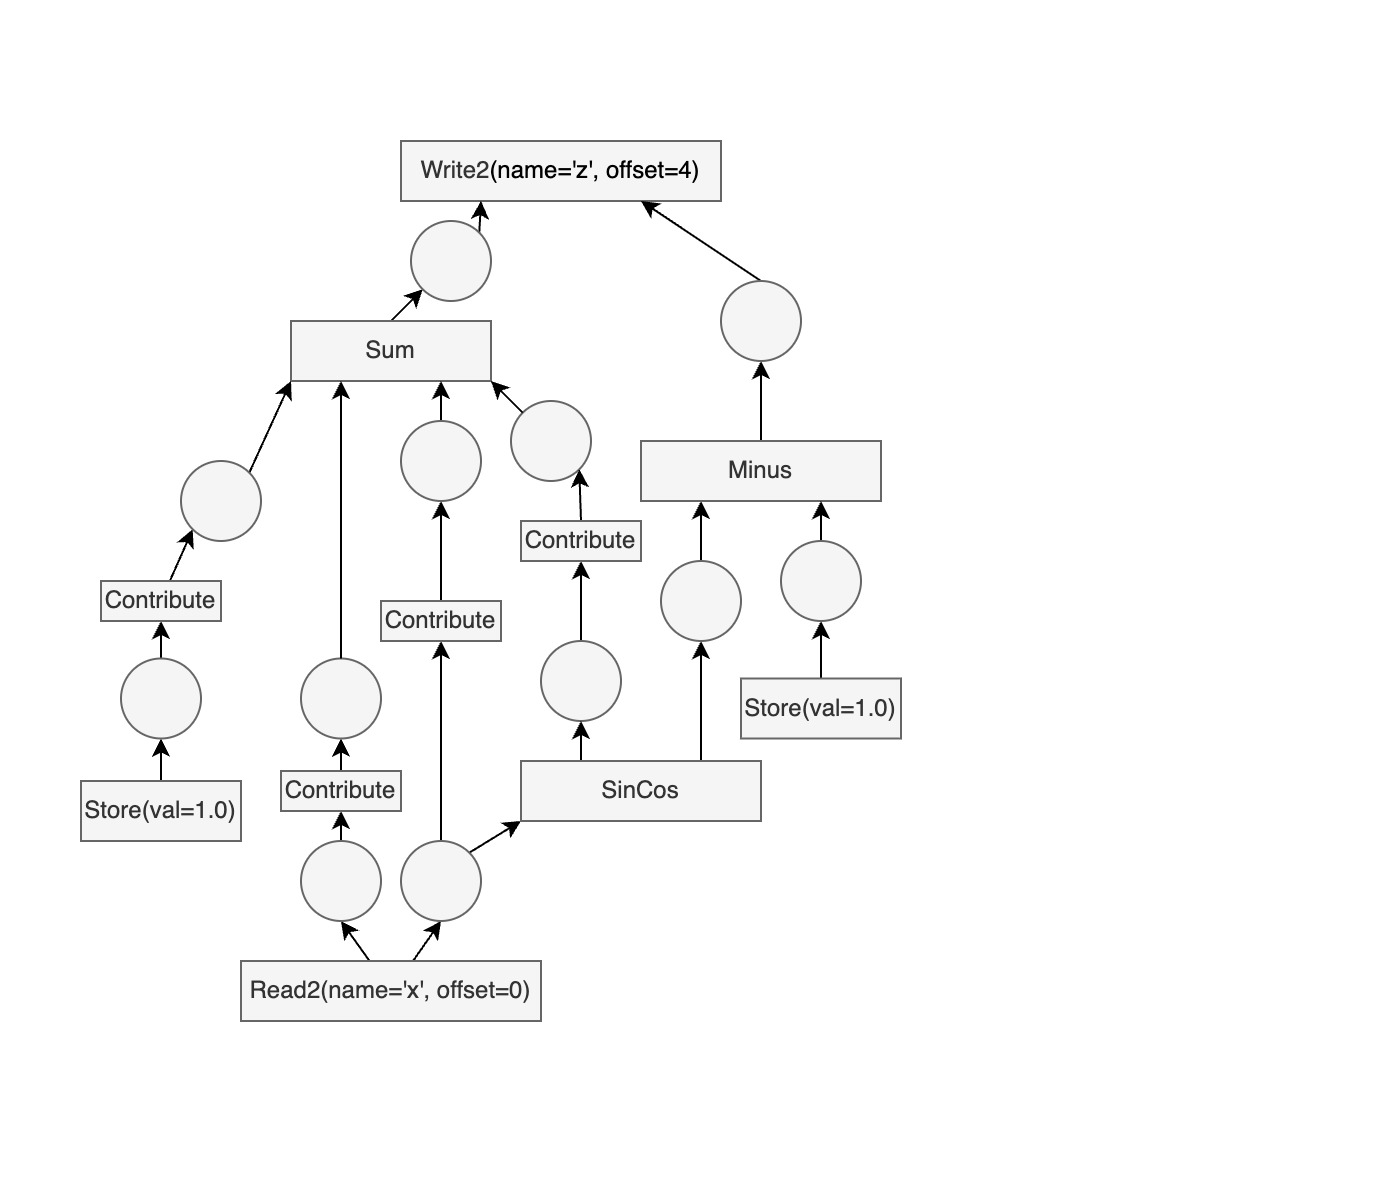
\includegraphics[trim={2.5cm 5cm 16cm 4cm},clip,width=0.5\textwidth]{figures/code_generation_example/symbolic_ordering-0.png}
        }
         &
        \subcaptionbox{Array of scalars}{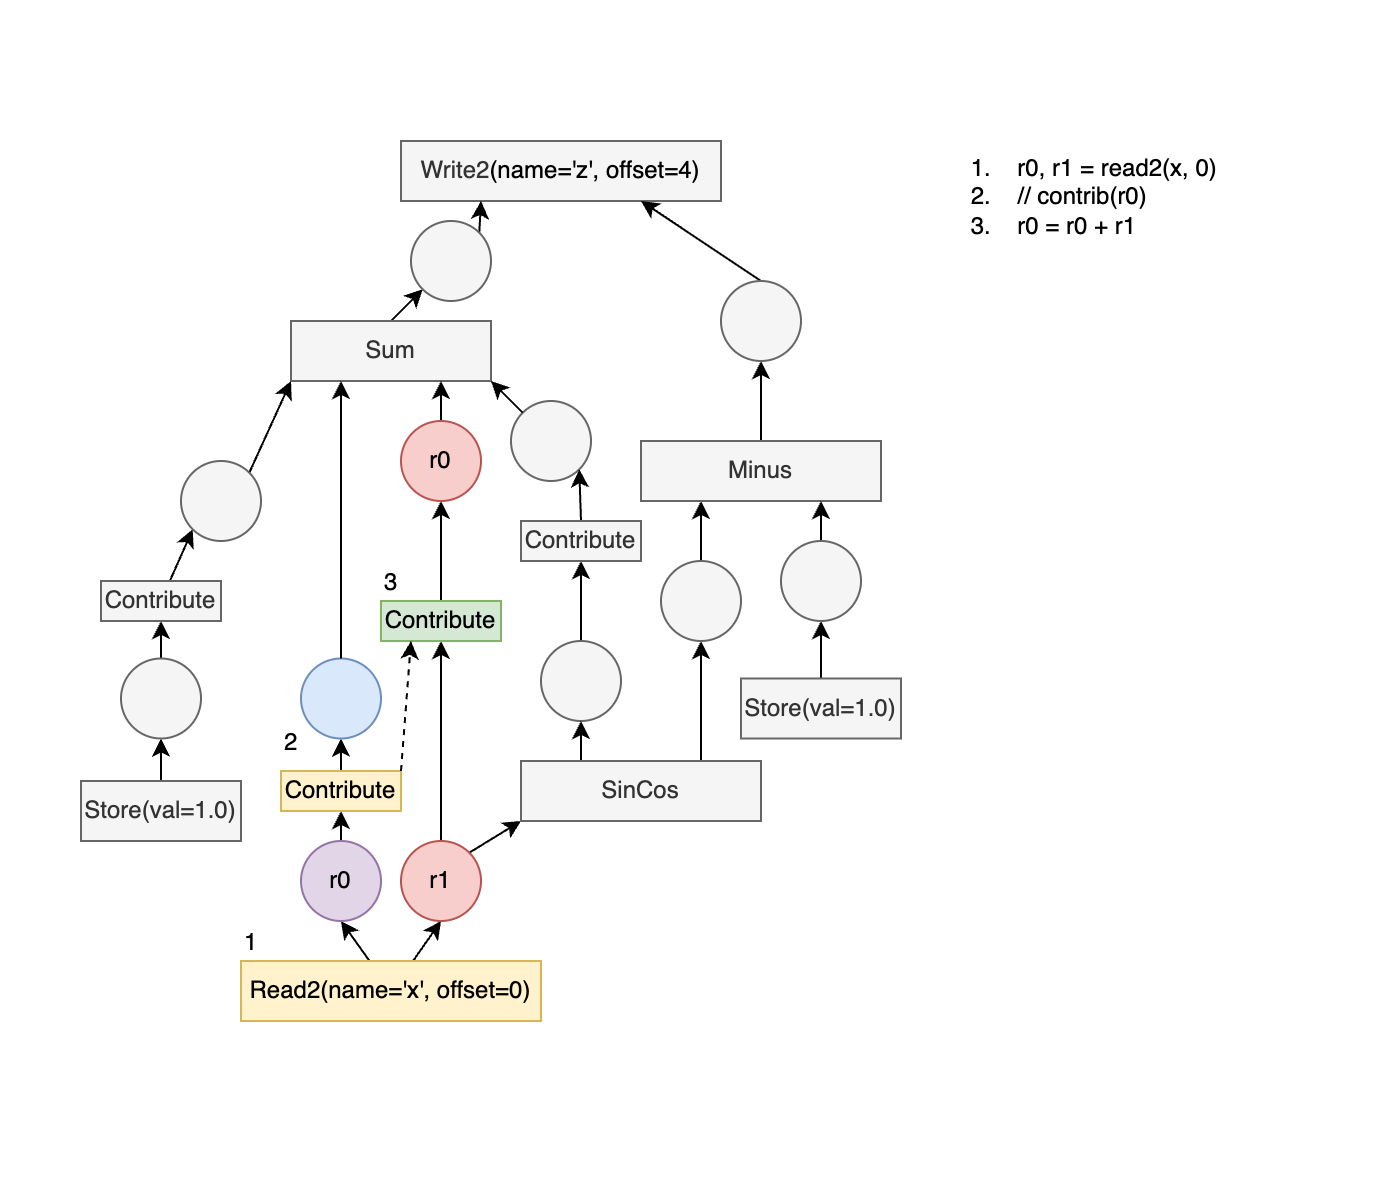
\includegraphics[trim={2.5cm 5cm 16cm 4cm},clip,width=0.5\textwidth]{figures/code_generation_example/symbolic_ordering-3.png}
        }
        \\ \vspace{0.5cm} \\
        \subcaptionbox{Array of scalars}{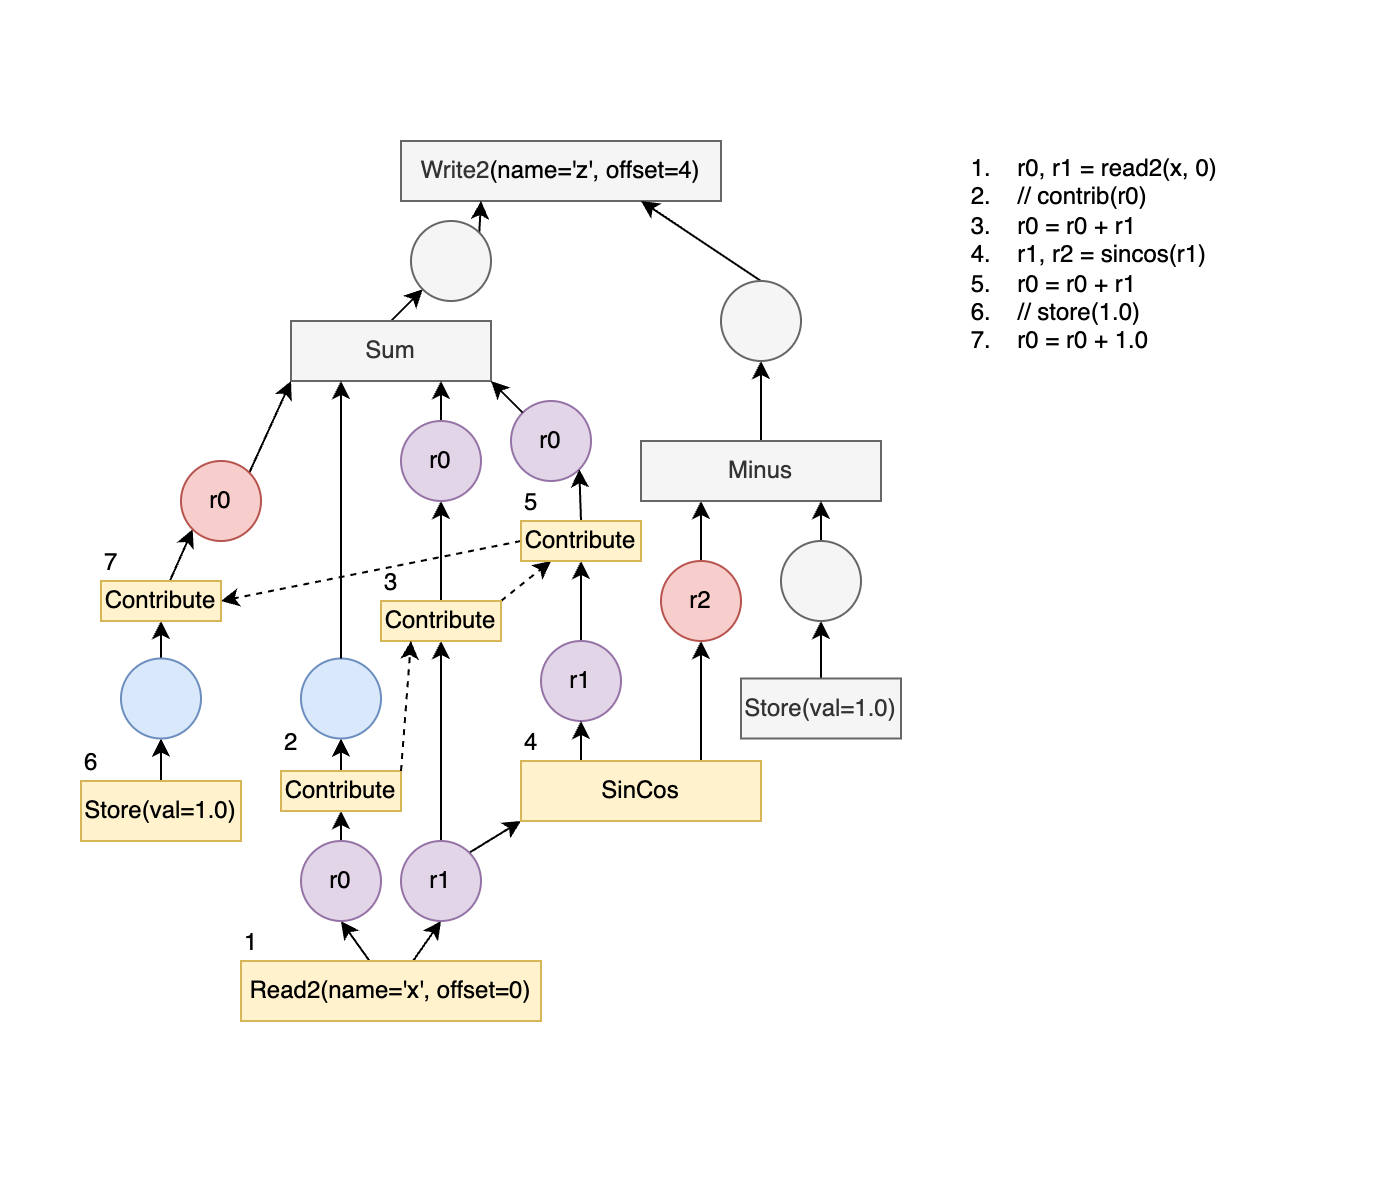
\includegraphics[trim={2.5cm 5cm 16cm 4cm},clip,width=0.5\textwidth]{figures/code_generation_example/symbolic_ordering-7.png}
        }

         &
        \subcaptionbox{Array of scalars}{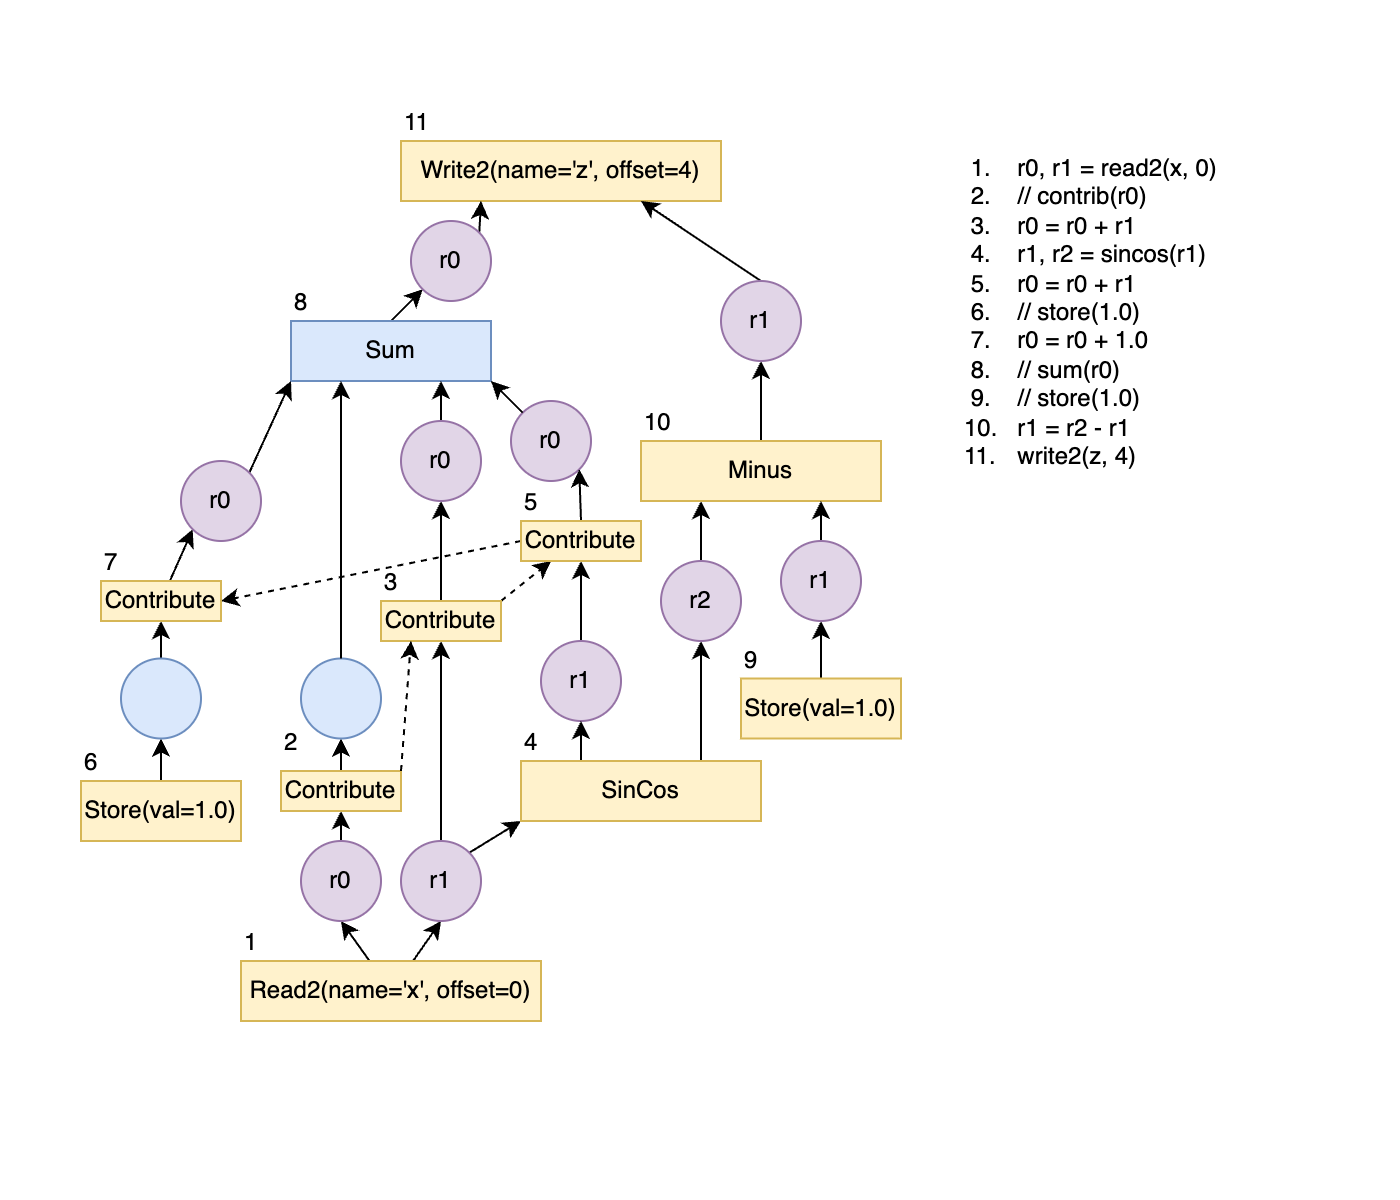
\includegraphics[trim={2.5cm 5cm 16cm 4cm},clip,width=0.5\textwidth]{figures/code_generation_example/symbolic_ordering-11.png}
        }

        \\
    \end{tabular}
    \caption{Mapping of arrays of structs with different number of fields. Fields are grouped into chunks of four as far as possibe, the remaning fields are appended at the end as chunks of the remaning size. All chunks are aligned to the number of bytes needed for the corresponding vector instruction.}
\end{figure}


\section{Memory Optimizations}

\section{Vector Instructions}
\cuda support vector accelerated memory operations of size 2, 3 and 4.
This means that we can load multiple values from memory in a single instruction.
This requires the data to be alagned to the size of the vector instruction.
For float instructions this is 8 bytes for float2 and 16 bytes for both float3 and float4.
As we also want acces patterns to be coalesced, we use the following memory layouts.


\begin{figure}[H]
    \centering
    \begin{tabular}[b]{ccc}
        \subcaptionbox{Array of scalars}{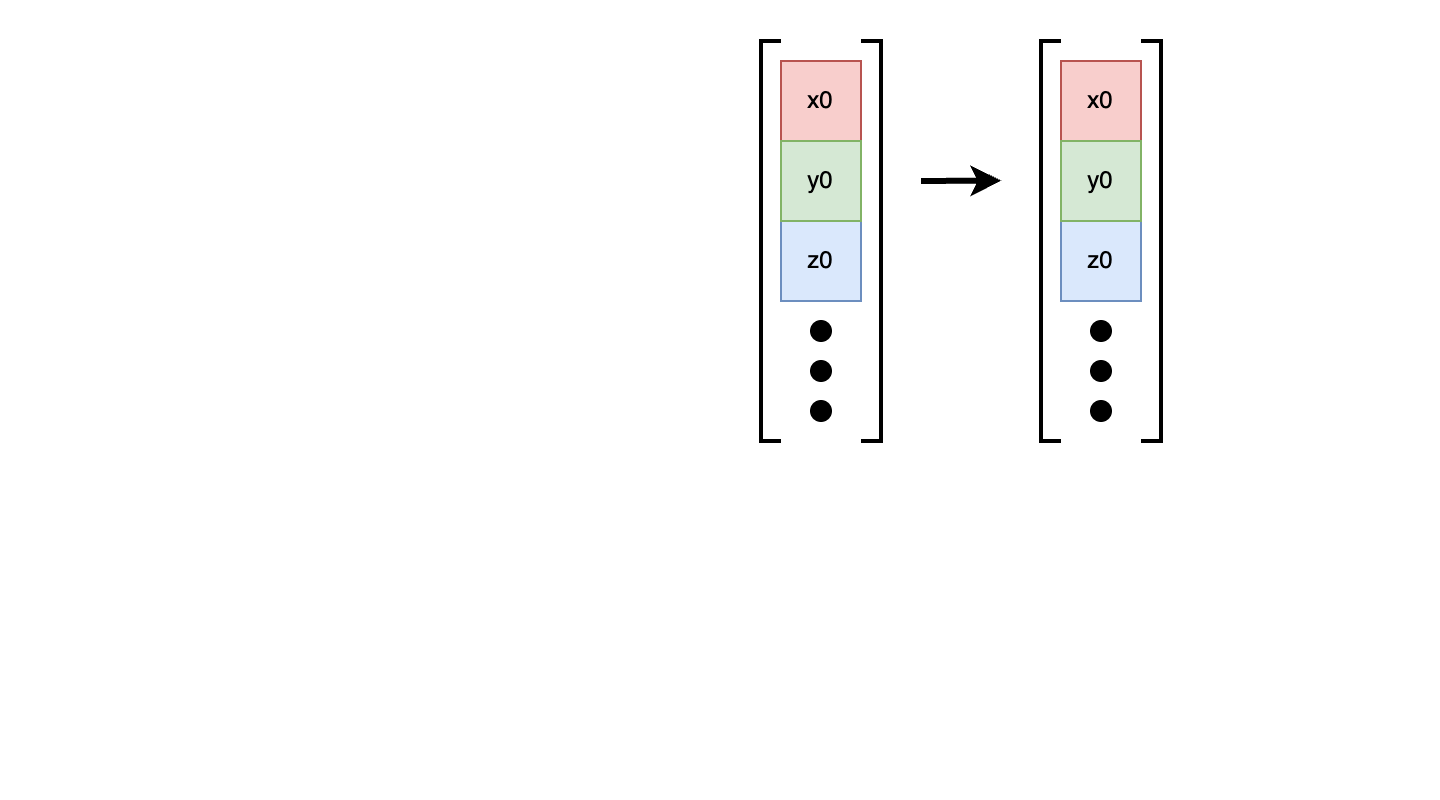
\includegraphics[trim={14cm 12cm -4cm 1cm},clip,width=0.5\textwidth]{figures/memlayouts/memlayout-1.png}
        } &
        \subcaptionbox{Array of structs with 3 fields.}{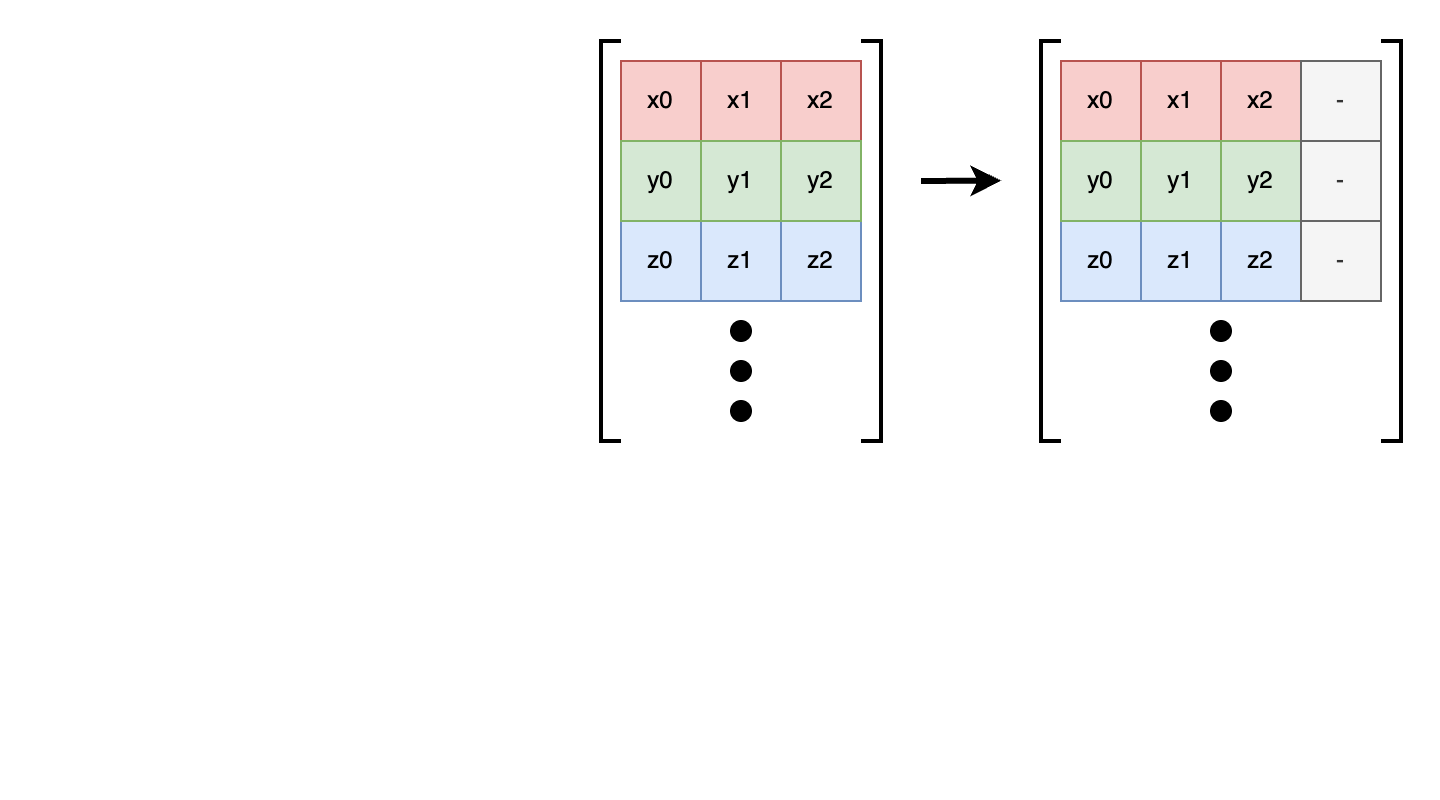
\includegraphics[trim={13cm 12cm -3cm 1cm},clip,width=0.5\textwidth]{figures/memlayouts/memlayout-3.png}
        }              \\
        \vspace{0.5cm} \\
        \subcaptionbox{Allay of structs with 6 fields.}{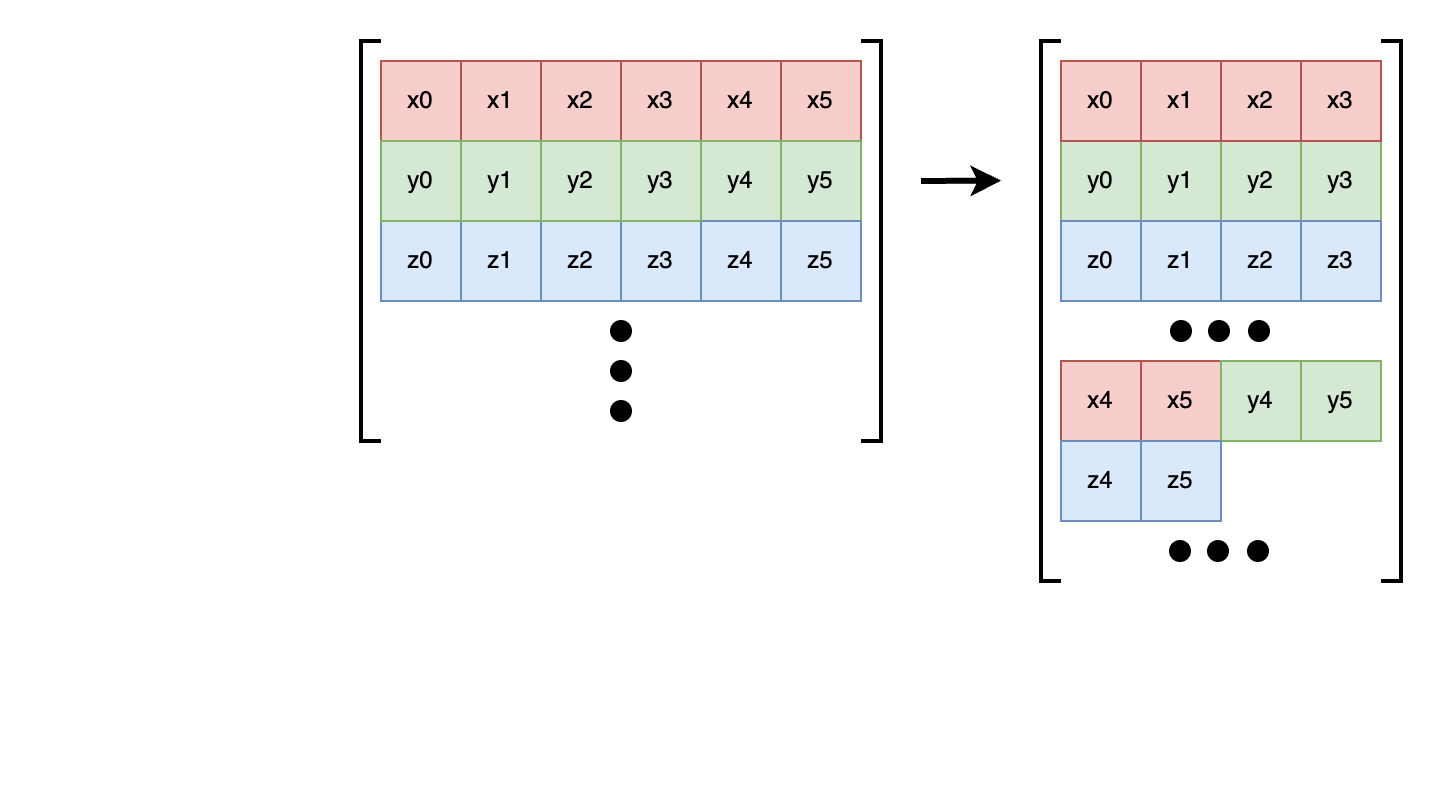
\includegraphics[trim={10cm 4cm 0cm 1cm},clip,width=0.5\textwidth]{figures/memlayouts/memlayout-6.png}
        } &
        \subcaptionbox{Array of structs with 7 fields.}{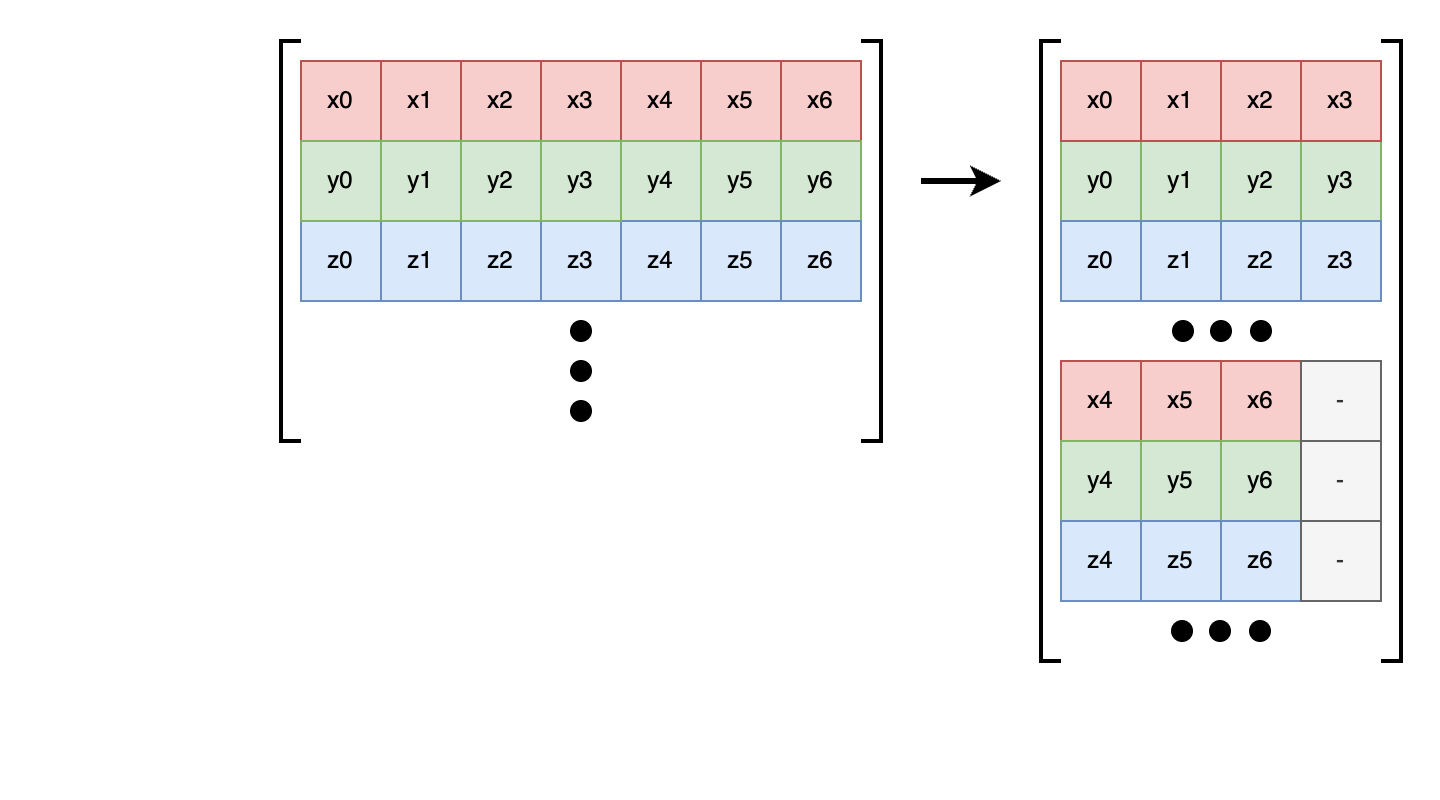
\includegraphics[trim={9cm 4cm 1cm 1cm},clip,width=0.5\textwidth]{figures/memlayouts/memlayout-7.png}
        }              \\
    \end{tabular}
    \caption{Mapping of arrays of structs with different number of fields. Fields are grouped into chunks of four as far as possibe, the remaning fields are appended at the end as chunks of the remaning size. All chunks are aligned to the number of bytes needed for the corresponding vector instruction.}
\end{figure}


\section{Access Patterns}
\subsection{Secuentual Acces}
\subsection{Indexed Acces}
\subsection{Shared Indexed Acces}

\subsection{Secuentual Add}
\subsection{Indexed Add}
\subsection{Shared Indexed Add}

\subsection{Unique Access}

\section{Solver Design}
Basacally just a copy of BAL.
Uses the same dampening update as everyone else.
Tried using \gls{cudss}

\subsection{Early Termination of PCGNR}
Unsucessfull steps are a waste of time.
Cost of \gls{pcgnr} iterations are significant compared to the cost of uptading estimates and evaluating the real cost function.
Check at regular intervls if we the real cost in decreasing.

Issue: Can lead to a low dampening factor and short steps.

\subsection{Kernel Fusion}
Every step of \gls{pcgnr} uses custiom \cuda kernels generated by \caspar
\section{Results}
\subsection{Bundle Adjustment in the Large Dataset}
Make graph plot of performance of ceres and caspar on the different bal datasets.


\section{Future Work}

\subsection{Improve Reordering Algorithm}
Currently performing only one greedy search. 
New method based on transactions?

\subsection{Incremental Solver}
Isn't freezing nodes faster?

\subsection{Constraint Handling}



\printbibliography

\end{document}